\documentclass[a4paper, 12pt]{article}%тип документа

%отступы
\usepackage[left=2cm,right=2cm,top=2cm,bottom=3cm,bindingoffset=0cm]{geometry}

%Русский язык
\usepackage[T2A]{fontenc} %кодировка
\usepackage[utf8]{inputenc} %кодировка исходного кода
\usepackage[english,russian]{babel} %локализация и переносы

%Вставка картинок
\usepackage{wrapfig}
\usepackage{graphicx}
\graphicspath{{pictures/}}
\DeclareGraphicsExtensions{.pdf,.png,.jpg}

%оглавление
\usepackage{titlesec}
\titlespacing{\chapter}{0pt}{-30pt}{12pt}
\titlespacing{\section}{\parindent}{5mm}{5mm}
\titlespacing{\subsection}{\parindent}{5mm}{5mm}
\usepackage{setspace}

%Графики
\usepackage{multirow}
\usepackage{pgfplots}
\pgfplotsset{compat=1.9}

%Математика
\usepackage{amsmath, amsfonts, amssymb, amsthm, mathtools}

%Стиль страницы
\usepackage{fancyhdr}
\pagestyle{fancy}

\begin{document}

\begin{titlepage}

\begin{center}
%\vspace*{1cm}
\large\textbf{Московский Физико-Технический Институт}\\
\large\textbf{(государственный университет)}
\vfill
\line(1,0){430}\\[1mm]
\huge\textbf{Работа 4.2.1}\\
\line(1,0){430}\\[1mm]
\vfill
\large Сибгатуллин Булат, ФРКТ\\
\end{center}

\end{titlepage}
\fancyhead[L] {Работа 4.2.1}
\noindent \textbf{Цель работы:} \\
\indent познакомиться с явлением интерференции в тонких пленках (полосы равной толщины) на примере колец Ньютона и с методикой интерференционных измерений кривизны стеклянной поверхности.\\
\noindent \textbf{В работе используются:} \\
\indent измерительный микроскоп с опак-иллюминатором; плоско-выпуклая линза; пластинка из черного стекла; ртутная лампа типа ДРШ; щель; линзы; призма прямого зрения; объектная шкала.

\section*{Экспериментальная установка}

На рис. 1. представлена схема наблюдения колец Ньютона. Найти радиус кривизны сферической поверхности такой линзы можно зная формулы для радиусов темных и светлых колец. Радиус темных колец:

\begin{equation} \label{bright}
r_m = \sqrt{m \lambda R}
\end{equation}

Радиус светлых колец:

\begin{equation}
r_m' = \sqrt{\frac{(m - 1) \lambda R}{2}}
\end{equation}

\begin{figure}[h!]
\centering
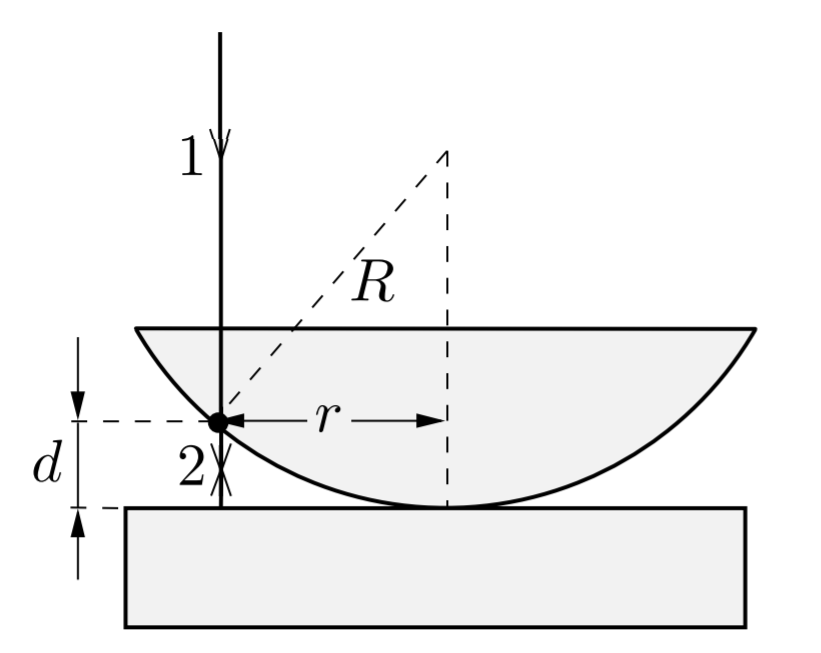
\includegraphics[scale=0.5]{images/scheme_0.png}
\caption{Схема наблюдения колец Ньютона}
\label{scheme_0}
\end{figure}

В нашей установке кольца Ньютона образуются при интерференции световых волн отраженных от границ тонкой воздушной прослойки заклюлченной между выпуклой поверхностью линзы и плоской стеклянной пластинкой.

Линии постоянной разности хода представляют собой концентрические кольца с центром в точке соприкосновения. Для протяженного источника линии равной толщины локализованы на поверхности линзы, если пластинка лежит на линзе, и вблизи поверхности линзы, если линза лежит на пластинке, как в нашем случае.

\vspace{0.5cm}

Схема экспериментальной установки представлена на рис. 1. Опыт выполняется с помощью измерительного микроскопа. На столике микроскопа помещается держатель с пластинкой черного стекла, на которой находится исследуемая линза.

\begin{figure}[h!]
\centering
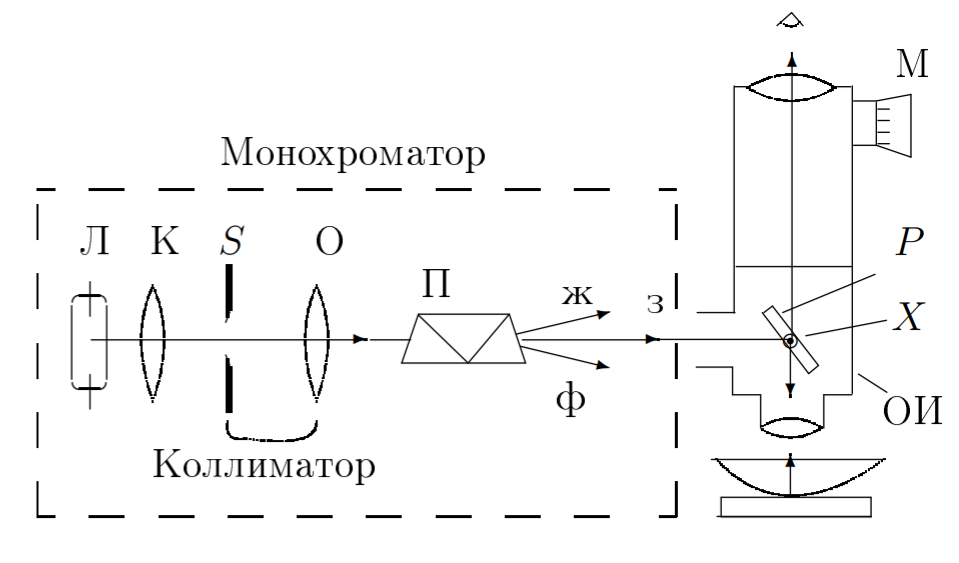
\includegraphics[scale=0.5]{images/scheme.png}
\caption{Схема установки для наблюдения колец Ньютона}
\label{scheme}
\end{figure}

Источником света служит ртутная лампа. Монохраматический свет получается в результате применения монохроматор, состоящий из конденсатора К, коллиматора (щель S и объектив O) и призмы прямого зрения П. Свет от монохроматора попадает на расположенный между объективом и окуляром микроскопа опак-иллюминатор (ОИ). Внутри опак-иллюминатора находится полупрозрачная стеклянная пластинка P, наколоненная под углом $45^{\circ}$ к оптической оси микроскопа. Свет частично отражается от этой пластинки, проходит через объектив и попадает на исследуемый объект.

Столик микроскопа может перемещаться в двух взаимно перпендикулярных направлениях с помощью винтов преперетоводителя. Отсчетный крест окулярной шкалы перемещается перпендикулярно оптической оси с помощью микроскопического винта М. Пластинка в опак-иллюминаторе может поворачиваться вокруг горизонтальной оси X, сам опак-иллюминатор  -- вокруг вертикальной оси.

\section*{Выполнение работы}

\begin{enumerate}

\item Настроим микроскоп и монохроматор так, чтобы в микроскоп было видно чередующиеся темные и светлые кольца. Вращая окулярный микрометрический винт убедимся, что перекрестие проходит через середину достаточно удаленного, но все еще отчетливо видимого тёмного кольца.

\item Перемещая перекрестие, будет последовательно устанавливать его на середины темных и светлых колец и записывать соответствующие показания окулярной шкалы и микрометра в таблицу:

\begin{center}
\begin{tabular}{|c|c|c|c|c|c|}
\hline 
 & \multicolumn{2}{c|}{Темные кольца} & & \multicolumn{2}{c|}{Светлые кольца} \\ 
\hline 
$m_{\text{тм}}$ & $l_{\text{ок}}$ & $l_{\text{мкм}}$ & $m_{\text{св}}$ & $l_{\text{ок}}$ & $l_{\text{мкм}}$ \\ 
\hline 
0 & 3 & 61 & 1 & 2 & 84 \\ 
\hline 
1 & 2 & 45 & 2 & 2 & 18 \\ 
\hline 
2 & 1 & 94 & 3 & 1 & 75 \\ 
\hline 
3 & 1 & 55 & 4 & 1 & 38 \\ 
\hline 
4 & 1 & 26 & 5 & 1 & 11 \\ 
\hline 
5 & 0 & 91 & 6 & 0 & 84 \\ 
\hline 
6 & 0 & 71 & 7 & 0 & 60 \\ 
\hline 
\end{tabular}
\end{center}

\item Произведем калибровку окулярной шкалы и рассчитаем цену ее деления. Получим, что цена деления окулярной шкалы равняется $\bigtriangleup l_{\text{ок}} \simeq 0,1 \textit{мм}$. Пользуясь полученным значением рассчитаем радиусы темных колец по формуле 

\[r_m = \mid l_{\text{ок} 0} - l_{\text{ок} m} + \frac{l_{\text{мкм} 0} - l_{\text{мкм} m}}{100} \mid \cdot \bigtriangleup l_{\text{ок}},\] 

аналогично рассчитаем радиусы светлых колец $r_m'$. Запишем получившиеся данные в таблицу:

\begin{center}
\begin{tabular}{|c|c|c|c|}
\hline 
 & Темные кольца & & Светлые кольца \\ 
\hline 
$m_{\text{тм}}$ & $l_{\text{тм}}$, мм &$m_{\text{св}}$ & $l_{\text{св}}$, мм \\ 
\hline 
0 & 0 & 1 & 0,077 \\ 
\hline 
1 & 0,116 & 2 & 0,143 \\ 
\hline 
2 & 0,167 & 3 & 0,186 \\ 
\hline 
3 & 0,206 & 4 & 0,223 \\ 
\hline 
4 & 0,235 & 5 & 0,250 \\ 
\hline 
5 & 0,270 & 6 & 0,277 \\ 
\hline 
6 & 0,290 & 7 & 0,301 \\ 
\hline 
\end{tabular} 
\end{center}

Погрешность цены деления будеем считать равной половине цены деления микрометра, то есть $\bigtriangleup l = 0,0005 \text{мм}$.

\item Построим график зависимости квадратов радиусов колец от их номера.

\begin{figure}[h!]
\centering
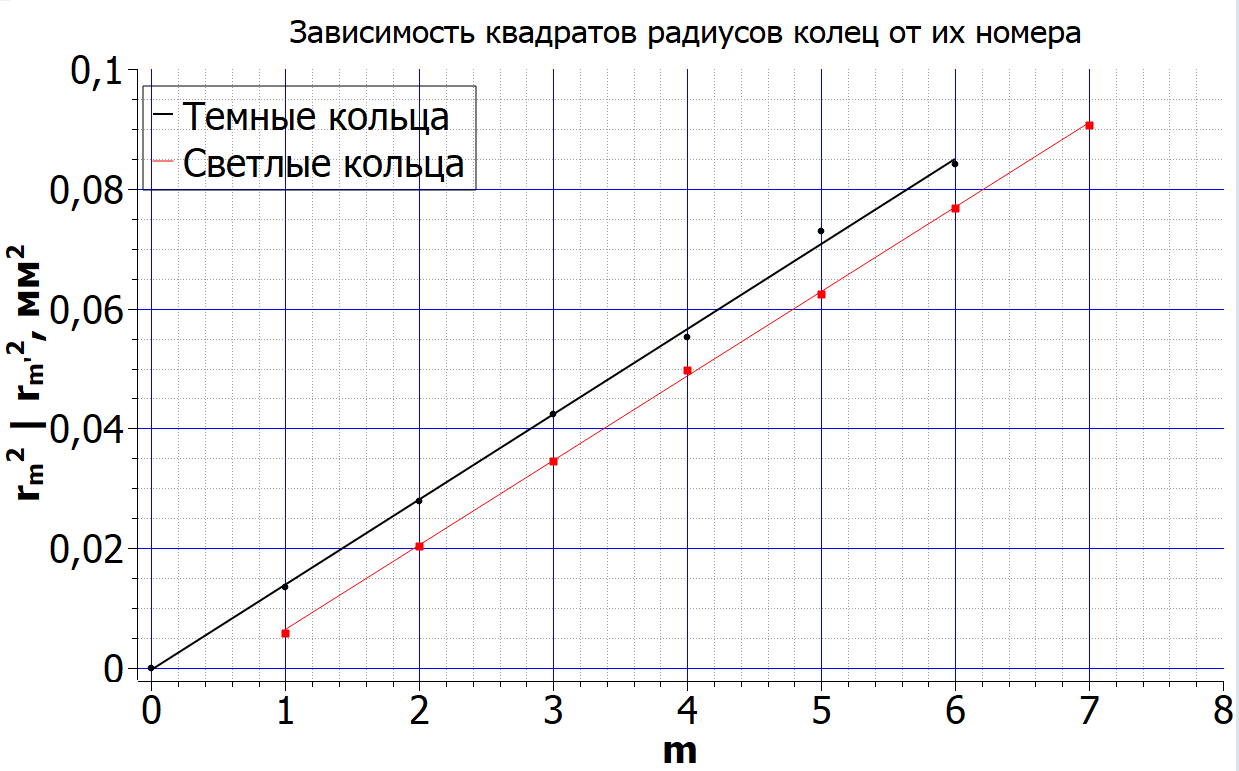
\includegraphics[scale=0.5]{images/graph_1.png}
\caption{График зависимости темных и светлых пятен от их номера}
\label{graph_1}
\end{figure}

Получим зависимость вида $y = a\cdot x + b$:

\begin{center}
\begin{tabular}{|c|c|c|}
\hline 
 & Темные кольца & Светлые кольца \\ 
\hline 
a & $0,0142\pm 0,0002$ & $0,0141\pm 0,0001$\\ 
\hline 
b & $-0,0004\pm 0,0008$ & $-0,0077\pm 0,0004$ \\ 
\hline 
\end{tabular} 
\end{center}

\item Расфокусировем монохроматор и получим в микроскопе изображение биений. Посчитаем количество темных полос от центра одной четкой системы полос, до другой: $\bigtriangleup m = 14$. Оценим разность длины волн по формуле:

\[(\bigtriangleup m + 1) \lambda_{\text{з}} = \bigtriangleup m \lambda_{\text{ж}} \Rightarrow \bigtriangleup \lambda = \frac{\lambda_{\text{з}}}{\bigtriangleup m} \simeq  39 \textit{нм},\]

здесь $\lambda_{\text{з}} = 546 \textit{нм}$. Теперь, подтвердив, что разность длин волн желтого и зеленого цвета: $\lambda_{\text{ж}} - \lambda_{\text{з}} \simeq 580 - 546 = 34$ примерно равны полученному нами значению, можем из графика посчитать радиус кривизны линзы $R$ по формуле $\eqref{bright}$:

\[a_{\text{св}} = \lambda \cdot R\]

Наконец получим значение для R:

\[R = \frac{a_{\text{св}}}{\lambda_{\text{з}}} = 2,60 \pm 0,04 \text{см}\]

\end{enumerate}

\section*{Вывод}

Таким образом, мы подтвердили, что лампа излучает свет зеленого цвета. В результате определения того, что разница длин волн желтого и зеленого света ртутной лампы примерно равна \fbox{$  \Delta \lambda = 39 \; нм $}, в то время как табличный результат --- 34 нм. Это может быть объяснено небольшой неточностью определения числа $ \Delta m $ из-за подрагиваний линзы, что осложняло подсчет колец с малой толщиной.
	
	Также мы построили графики зависимости радиусов колец Ньютона от их номеров. Полученный результат позволил нам рассчитать радиус линзы ---  \fbox{$ R = (2,60 \pm 0,04) \; см $}.

\end{document} 